%------------------------------------------------------------------------------
% Template file for the submission of papers to IUCr journals in LaTeX2e
% using the iucr document class
% Copyright 1999-2013 International Union of Crystallography
% Version 1.6 (28 March 2013)
%------------------------------------------------------------------------------


% \documentclass[preprint]{iucr}
\documentclass{iucr}


\usepackage{siunitx}
\usepackage{color}
% \usepackage{amsmath,amssymb}
% \usepackage{amsfonts} 
\usepackage{mathtools}
\usepackage[normalem]{ulem}
% rotation table labels...
% see https://tex.stackexchange.com/questions/98388/how-to-make-table-with-rotated-table-headers-in-latex
\usepackage{adjustbox}
\usepackage{array}
\usepackage{booktabs}
\usepackage{multirow}

\usepackage{amsmath}
\usepackage{url}

%%%%%%%%%%%%%%%%
\usepackage[utf8]{inputenc}
\usepackage[]{graphicx}
\usepackage{rotating}
\usepackage{hyperref}
\usepackage{listings}

% \lstset{basicstyle=\small,
% % keywordstyle=\bf \color{blue},
% % identifierstyle=\underline,
% % commentstyle=\color[red]{0.5},
% stringstyle=\ttfamily \color{red},
% showstringspaces=false}
\lstset{language=Fortran,
        keywordstyle=\color{blue}\textbf,
	commentstyle=\color[rgb]{0.133,0.545,0.133},
	stringstyle=\color[rgb]{0.627,0.126,0.941},
	breaklines=true,
	showstringspaces=false,
	frame=trBL, basicstyle=\scriptsize %\small %\tiny %\footnotesize
       }
%%%%%%%%%%%%%%%%



% \usepackage{enumitem}
% \usepackage[normalem]{ulem}
% % srio..........
% \usepackage{multicol}
% \usepackage{graphicx}
\DeclareMathOperator{\sinc}{sinc}

\newcommand{\todo}[1]{{\color{red}[TODO: "#1'']}}
\newcommand{\remove}[1]{ {\color{blue} \sout{#1}}}
\newcommand{\inblue}[1]{{\color{blue}#1}}
\newcommand{\inred}[1]{{\color{red}#1}}
\newcommand{\ingreen}[1]{{\color{green}#1}}
\newcommand{\soutred}[1]{{\color{red}\sout{#1}}}
\newcommand{\lambdabar}{{\mkern0.75mu\mathchar '26\mkern -8.2mu\lambda}}

\definecolor{JSR_blue}{RGB}{51, 102, 154}
\newcommand{\jsrblue}[1]{\textcolor{JSR_blue}{#1}}

\newcolumntype{R}[2]{%
    >{\adjustbox{angle=#1,lap=\width-(#2)}\bgroup}%
    l%
    <{\egroup}%
}
\newcommand*\rot{\multicolumn{1}{R{90}{1em}}
}
%in preprint use 
% \newcommand{\whencolumns}[2]{#1}
% otherwise
% \newcommand{\whencolumns}[2]{#2}

\makeatletter
\@ifclasswith{iucr}{preprint}{
\newcommand{\whencolumns}[2]{#1}
}{
\newcommand{\whencolumns}[2]{#2}
}
\makeatother


 %-------------------------------------------------------------------------
 % Information about journal to which submitted
 %-------------------------------------------------------------------------
 \journalcode{X}              % Indicate the journal to which submitted
                              %   A - Acta Crystallographica Section A
                              %   B - Acta Crystallographica Section B
                              %   C - Acta Crystallographica Section C
                              %   D - Acta Crystallographica Section D
                              %   E - Acta Crystallographica Section E
                              %   F - Acta Crystallographica Section F
                              %   J - Journal of Applied Crystallography
                              %   M - IUCrJ
                              %   S - Journal of Synchrotron Radiation



\begin{document}                  % DO NOT DELETE THIS LINE

% \if@twocolumn
% \newcommand{\whencolumns}[2]{
% #2
% }
% \else
% \newcommand{\whencolumns}[2]{
% #1
% }
% \fi
% \makeatother

\title{Ray tracing simulations of X-ray polarizers and phase-shifters. The SHADOW4 models to transport and modify electric fields.}

\cauthor[1]{\jsrblue{Manuel}}{\jsrblue{Sanchez del Rio}}{srio@esrf.eu}{address if different from \aff}
\author[1]{\jsrblue{Juan}}{\jsrblue{Reyes-Herrera}}
\author[2]{\jsrblue{Xiaojian}}{\jsrblue{Yu}}

\aff[1]{ESRF - The European Synchrotron, 71 Avenue des Martyrs, 38000 Grenoble, \country{France}}
\aff[2]{Singapore Synchrotron Light Source,National University of Singapore, 5 Research Link, Singapore 117603 \country{Singapore}}

\maketitle                        % DO NOT DELETE THIS LINE

% -----------------------------------------------------------------
% -----------------------------------------------------------------

\begin{synopsis}
We explain how SHADOW manipulates the electric vectors. We present some examples of simulations on X-ray polarizers and phase shifters. 
\end{synopsis}

% -----------------------------------------------------------------
% -----------------------------------------------------------------

\begin{abstract}
We explain here the models implemented in the SHADOW4 ray tracing code to modify and transport the electric fields and related parameters (intensity, polarization). We show some examples of X-ray polarizers and phase shifters.
\end{abstract}

% -----------------------------------------------------------------
% -----------------------------------------------------------------
\section{Introduction}
\label{sec:introduction}
% -----------------------------------------------------------------
% -----------------------------------------------------------------

Ray tracing simulations serve as essential tools for designing, optimizing, and analyzing optical systems, providing invaluable insights into how light rays propagate through intricate arrangements of optical components. Here, we look to the optical devices that change the polarization state of the beam. In order to simulate them, each ray carries information on the electric field and phase. These are transported along the beamline, and modified by the optical elements. We describe the models used to do that. 

SHADOW, in its first version SHADOW1 \cite{Cerrina1984} already incorporated a full description of the electrid field and phases.
In fact, the two components of the electric field ($\pi$ or ``parallel" to the scattering or diffraction plane, and $\sigma$ or ``perpendicular" to the scattering plane) are defined for each ray. 
This allowed the correct, or ``polarized" treatement of the reflections in mirrors. SHADOW2 \cite{Lai1988} included a model for plane crystals in Bragg (or reflection) geometry.
This model was further upgraded to include asymmetric crystals \cite{SanchezdelRio1992}, and crystals in transmission or Laue geometry \cite{SanchezdelRio1994}.
In SHADOW3 \cite{codeSHADOW} and its ShadowOui \cite{codeSHADOWOUI} interface, the definition of the crystal parameters was done in a more user friendly way, also incorporating the posibility to use external diffraction profiles.
At this point, SHADOW allows for simulation of a great number of crystal devices, including
\begin{itemize}
    \item the classic reflection by a flat perfect crystal in symmetric or asymmetric configurations. This includes most types of X-ray monochromators included in the beamlines (channel cut, double-crystal monochromators, high resolution nested monochromators, etc.)
    \item curved crystals in both Johan and Johansson configurations, with different shapes. For example, elliptically bent Bragg crystals used in X-ray polychromators in dispersive-EXAFS beamlines, or spherical crystal analyzers. Note that the internal calculation of the crystal reflectivity is done by SHADOW considered the crystal undistorted. If the curvature induces a high distortion in the crystal, the reflectivity profiles is modified and the internal calculation mode is not accurate. In this case, an external profile calculated in OASYS/XOPPY can be used, but this works only for symmetric Bragg crystals.
    \item some cases of Laue crystals. For example, flat Laue crystals that present a sort of ``polychromatic focusing". The case of full bent crystal is not allowed because i) the reflectivity curve calculated internally is for the undistorted crystal (in many cases Laue monochromators exploit the fact that the diffraction wisth is increased when bending); ii) some effects predicted by the Dynamical theory of diffraction are not considered in the ray tracing model, like the focusing of the Bormann triangle, and the correct focusing of the beam due to the splerical nature of the diffracted waves. 
    \item the case of the crystal polarized using flat crystals at Bragg angle of $\theta_B$=\SI{45}{\deg} where the $\pi$ reflectivity is zero. However, in cases where the ``purity" of the polarization has to be calculated, the necessity of using very small numbers may induce o numerical imprecissions. This will be discussed in one of the examples presented. 
    \item we recall that the dynamical theory predicts two waves for crystals in both Bragg or Laue geometries: the diffracted and the transmitted. SHADOW3 always use the diffracted beam. This is a limitation for calculating phase-shifters, that are typically flat crystals set close but not exactly at the Bragg angle, but using the transmitted beam that shows an important change in the polarization state. This is now possible with SHADOW4 using the new elements ``crystal phase plates" \todo{not yet available}.
    \item SHADOW can consider multiple crystal structures already available in the databases, as for example some crystals interesting for tender X-rays, like YB$_{66}$ of Muscovite \cite{Yu_2022}. In general, there is a procedure to introduce the crystal lattice and unit cell parameters to implement a new crystal. 
\end{itemize}


With the advent of SHADOW4 \cite{ShadowSRN2023}, a new refactoring, and refurbishing of this popular ray tracing code, we have changed, revisited, reimplemented, and improved in several ways, the methods used to transport and modify by optical elements the electric fields. This allows to increase the performances of the simulations that become more accurate.
This paper aims to describe the methods and algorithms used in SHADOW4 for modifying the electric fields with special emphases in crystal optics and its use for X-ray polarisers.   

Most Monte-Carlo codes store a parameter ``intensity'' or weight for each ray that allow to track the energy or intensity of each traced event.
As most of electromagnetic interactions are better described by the change in the electric field, it is more appropriated to store directly the electric fields and not the intensity. 
The intensity is the square of the electric field modulus.
The electric fields permit not only to compute intensity or each ray, but also the polarization, phase changes, and coherence properties.
In order to extract usable and accurate information on these important parameters, the electric fields must be correctly simulated and propagated.
We summarize here some of the assumptions and manipulations of the electric fields in SHADOW. 

% % -----------------------------------------------------------------
% -----------------------------------------------------------------
\section{SHADOW arrays and description of the electric field}
\label{sec:definitions}
% -----------------------------------------------------------------
% -----------------------------------------------------------------



A single ray $\vec{R}$ in SHADOW is an array of 18 parameters (called ``columns'' in SHADOW's jargon) stored in the following order:
\begin{equation}
   \vec{R}=( \vec{x},\vec{v},\vec{E}_\sigma,f,k,n,opd,\phi_\sigma,\phi_\pi,\vec{E}_\pi)
\end{equation}
where $\vec{x}=(x_1,x_2,x_3)^T$ ($T$ is the transpose operator) are the spatial coordinates, $\vec{v}=(v_1,v_2,v_3)^T$ the director cosines (ray direction) with $|\vec{v}|=1$, $f$ is a flag (good or lost ray), $k$ is the wavevector modulus in $cm^{-1}$ ($k=2\pi / \lambda$, with $\lambda$ the photon wavelength ), $n$ is a counter (from one to the total number of rays), $opd$ is the optical path (the travelled distance times the refraction index).
The complex electric vector is expressed as a function of the $\sigma$ and $\pi$ components (perpendicular and parallel to the diffraction of reflection plane, respectively):

\begin{equation}\label{eq:electricfieldray}
   \vec{E}= \vec{E}_\sigma e^{i \phi_\sigma} + \vec{E}_\pi e^{i \phi_\pi}.
\end{equation}

The storage in SHADOW is redundant, which imply that some relationships among the parameters must hold. For example, being the direction a unitary vector, $v_3\text{=}\sqrt{v_1^2+v_2^2}$. Concerning the electric fields,
\begin{itemize}
 \item $\vec{E}_\sigma \perp \vec{E}_\pi$, $\vec{E}_\sigma \perp \vec{v}$, $\vec{E}_\pi \perp \vec{v}$
 \item $\vec{E}_\sigma$ and $\vec{E}_\pi$ are real
 \item $|\vec{E}|^2=1$ at the source, and $|\vec{E}|$ is reduced as far as the ray interacts with the different 
 optical elements
\end{itemize}

The intensity carried-out by a single ray is:
\begin{eqnarray}
   I=|\vec{E}|^2 = \vec{E}.\vec{E}^* = (\vec{E}_\sigma e^{i \phi_\sigma} + \vec{E}_\pi e^{i\phi_\pi} ).
   (\vec{E}_\sigma e^{-i\phi_\sigma} + \vec{E}_\pi e^{-i\phi_\pi} ) =  \nonumber \\
   |\vec{E}_\sigma|^2 + |\vec{E}_\pi|^2 + 2 \vec{E}_\sigma.\vec{E}_\pi \cos(\phi_\sigma-\phi_\pi) =
   |\vec{E}_\sigma|^2 + |\vec{E}_\pi|^2.
\end{eqnarray}


% -----------------------------------------------------------------
% -----------------------------------------------------------------
\section{The electric fields at the source}
\label{sec:source}
% -----------------------------------------------------------------
% -----------------------------------------------------------------

When simulating a source, SHADOW first samples the ray energy, direction and positions and then define set electric vectors. 
A first step is to obtain orthogonal unitary vectors $\vec{u}_\sigma$ and $\vec{u}_\pi$ normal to $\vec{v}$. At the source 
level, there is not yet knowledge of any optical surface to define $\sigma$ and $\pi$ directions, so these directions 
are considered ``mostly'' horizontal and vertical, respectively. The unitary vectors are calculated as: 
\begin{eqnarray}
   \vec{u}_\sigma = \vec{v} \wedge (\vec{u}_1 \wedge{v}) \nonumber \\
   \vec{u}_\pi = \vec{u}_\sigma \wedge  {v}
\end{eqnarray}
with $\wedge$ the cross product, and  $\vec{u}_1\text{=}(1,0,0)$ the unitary vector along the horizontal direction at the source plane ($x$ axis).
This is done for most SHADOW4 sources by using the {\tt vector\_default\_efields} function found in {\tt shadow4.tools.arrayofvectors} (see listing \ref{lst:vectordefaultefields}).

\begin{lstlisting}[caption={\it Function {\tt vector\_default\_efields} used to create electric vectors $\sigma$ and $\pi$ perpendicular to a given direction and with a given polarization dregree}, label={lst:vectordefaultefields}, captionpos=b]
def vector_default_efields(DIREC, pol_deg=1.0):
    # Generates the normalized electric vectors perpendicular to DIREC
    # This is defined on the source plane, so that A_VEC is along the X-axis and AP_VEC is along Z-axis.
    # Then care must be taken so that A will be perpendicular to the ray direction.

    A_VEC = numpy.zeros_like(DIREC)
    A_VEC[:, 0] = 1.0

    # ! C   Rotate A_VEC so that it will be perpendicular to DIREC and with the
    # ! C   right components on the plane.
    A_TEMP = vector_cross(A_VEC, DIREC)
    A_VEC = vector_cross(DIREC, A_TEMP)
    A_VEC = vector_norm(A_VEC)
    AP_VEC = vector_cross(A_VEC, DIREC)
    AP_VEC = vector_norm(AP_VEC)

    #
    # obtain polarization for each ray (interpolation)
    #
    DENOM = numpy.sqrt(1.0 - 2.0 * pol_deg + 2.0 * pol_deg ** 2)
    AX = pol_deg / DENOM
    for i in range(3):
        A_VEC[:, i] *= AX

    AZ = (1.0 - pol_deg) / DENOM
    for i in range(3):
        AP_VEC[:, i] *= AZ

    return A_VEC, AP_VEC

\end{lstlisting} 

Then the electric vectors are these versors times the corresponding ($\sigma$ or $\pi$) modulus, in such a way that  the intensity is one. The mudulus of each component is a function of a {\it particular}\footnote{In SHADOW the polarization is defined as a function of the amplitudes and not the intensities, in such a way that $P=|\vec{E}_\sigma|/(|\vec{E}_\sigma|+|\vec{E}_\pi|)$} polarization degree defined as:
\begin{equation}
   P = \frac{\cos \chi}{\cos \chi + \sin \chi}
\end{equation}
where $\chi$ is the angle between $\vec{E}_\sigma$ and $\vec{u}_1$ when the beam is linearly polarized. 
The electric vector components are: 
\begin{eqnarray}
   \vec{E}_\sigma = \frac{P}{\sqrt{1-2 P+ 2 P^2}} \vec{u}_\sigma \nonumber \\
   \vec{E}_\pi    = \frac{1-P}{\sqrt{1-2 P+ 2 P^2}} \vec{u}_\pi.
\end{eqnarray}
These expressions verify, as expected,  $|\vec{E}_\sigma|^2 + |\vec{E}_\pi|^2 = 1$, and $P=|\vec{E}_\sigma|/(|\vec{E}_\sigma|+|\vec{E}_\pi|)$



The phase $\phi_\sigma$ is set to zero for coherent beams or to a random angle in $[0,360^{\circ})$ for an incoherent beam, and
$\phi_\pi=\phi_\sigma+\Phi$ with: 
\begin{itemize}
 \item $\Phi=0$ for linearly polarizad light 
 \item $\Phi=90^{\circ}$ for right (CW) elliptical polarization
 \item $\Phi=-90^{\circ}$ for left (CCW) elliptical polarization.
\end{itemize}
A few examples: 
\begin{itemize}
 \item $P=1$,$\Phi=0$ for horizontal linearly polarizad light 
 \item $P=0$,$\Phi=0$ for vertical linearly polarizad light
 \item $P=0.5$,$\Phi=0$ for $45^\circ$ linearly polarizad light
 \item $P=0.5$ $\Phi=90^{\circ}$ for right circular polarization
 \item $P<0.5$,$\Phi=-90^{\circ}$ for left elliptical polarization mostly horizontal
\end{itemize}


\section{Change of reference frame}
\label{sec:change_frame}

xxxxx

\begin{figure}
\label{fig:S4_reference_frame}
    \centering
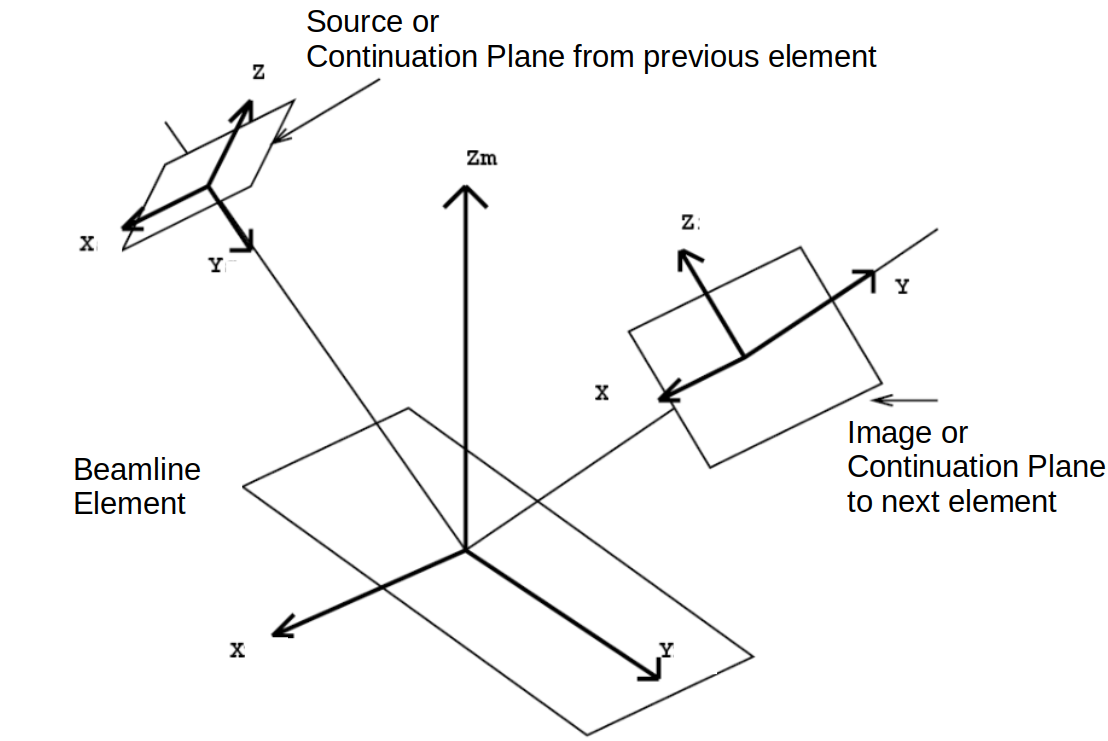
\includegraphics[width=0.9\linewidth]{figures/S4_reference_frame.png}
\caption{SHADOW4 reference frame definitions: Source, beamline element, and image coordinates.}  
\end{figure}

The beam coming from the source or a previous beamline element must be converted into the reference frame of the o.e. for performing the ray tracing.
The rotation of the vectors from the beam is done in the method {\tt S4beam.rotate()}.
It rotates the beam around one of its principal axis.
In SHADOW4 the ``beamline element" is formed by an ``optical element" object and a ``coordinates" object containing two angles: the incidence angle $\theta$ and the beamline element orientation angle $\alpha$, and two distances: the distance $p$ from the source (or continuation plane from the previous element), and $q$ from the beamline element to its image plane or continuation plane.
Therefore, the beam vectors $\vec{x}$,  $\vec{v}$ and $\vec{E}_{\sigma,\pi}$ must be rotated sequentially:
\begin{itemize}
    \item by an angle $\alpha$ around the $y$ axis, 
    \item an by an angle $\theta_i$ around the $x$ axis,
\end{itemize}
and then the beam coordinates $\vec{x}$ translated a distance $-p$. 

An example of code is the following, found in the method {\tt trace\_beam()} of the beamline element (see listing~\ref{lst:changereferencetobeamlineelement})

\begin{lstlisting}[caption={\it Piece of code that changes the beam from the source reference frame to the local beamline element frame.}, label={lst:changereferencetobeamlineelement}, captionpos=b]
        #
        # put beam in mirror reference system
        #
        input_beam.rotate(alpha1, axis=2)
        input_beam.rotate(theta_grazing1, axis=1)
        input_beam.translation([0.0, -p * numpy.cos(theta_grazing1), p * numpy.sin(theta_grazing1)])
\end{lstlisting}

Then, the reflection/refraction/diffraction by the beamline element is applied, which changes the beam direction and electric vectors.
{\bf This will be discussed in detail in the next paragraphs}.

Last, after the reflection, the rays are 
\begin{itemize}
    \item projected into the image plane, and
    \item change the coordinate system to have the origin in the image plane.
\end{itemize}
For that it projects the  vectors onto the versors of the new reference. 
These operations are done by the method {\tt change\_to\_image\_reference\_system} of {\tt S4beam} (see listing~\ref{lst:changetoimagereferencesystem}).

\begin{lstlisting}[caption={\it Method of {\tt S4Beam} that changes the reference and propagates the beam from the beamline element to the image plane.}, label={lst:changetoimagereferencesystem}, captionpos=b]
   def change_to_image_reference_system(self, theta, T_IMAGE, rad=True,
            refraction_index=1.0,
            apply_attenuation=0,
            linear_attenuation_coefficient=0.0, # in SI, i.e. m^-1
            ):
        """
        Implements the propagation from the mirror reference frame to the screen (image) reference.
        Mimics IMREF and IMAGE1 subrutines in shadow3

        Parameters
        ----------
        theta: float
            the grazing angle in rad (default) or deg (if deg=False).
        T_IMAGE: float
            the distance o.e. to image in m.
        rad: boolean, optional
            set False if theta is given in degrees.
                refraction_index
        apply_attenuation : int, optional
            A flag to indicate that attenuation must be applied (using linear_attenuation_coefficient).
        linear_attenuation_coefficient : float or numpy array
            The attenuation coefficient in m^(-1).
        """
        if rad:
            theta1 = theta
        else:
            theta1 = theta * numpy.pi / 180

        T_REFLECTION = numpy.pi / 2 - theta1

        a1 = self.rays.copy()

        nrays = self.rays.shape[0]
        UXIM_x = numpy.ones(nrays)
        UXIM_y = numpy.zeros(nrays)
        UXIM_z = numpy.zeros(nrays)

        VZIM_x = numpy.zeros(nrays)
        VZIM_y = numpy.zeros(nrays) - numpy.cos(T_REFLECTION)
        VZIM_z = numpy.zeros(nrays) + numpy.sin(T_REFLECTION)

        VNIMAG_x = numpy.zeros(nrays)
        VNIMAG_y = numpy.zeros(nrays) + numpy.sin(T_REFLECTION)
        VNIMAG_z = numpy.zeros(nrays) + numpy.cos(T_REFLECTION)

        ABOVE = T_IMAGE - a1[:,0] * VNIMAG_x - a1[:,1] * VNIMAG_y - a1[:,2] * VNIMAG_z
        BELOW = VNIMAG_x * a1[:,3] + VNIMAG_y * a1[:,4] + VNIMAG_z * a1[:,5]

        DIST = ABOVE / BELOW

        failure = numpy.argwhere(BELOW == 0)
        if len(failure) > 0:
            a1[failure, 9] = -3.0e-6

        # ! ** Computes now the intersections onto TRUE image plane.
        a1[:, 0]  +=   DIST * a1[:, 3]
        a1[:, 1]  +=   DIST * a1[:, 4]
        a1[:, 2]  +=   DIST * a1[:, 5]

        #!  ** Rotate now the results in the STAR (or TRUE image) reference plane.
        #!  ** Computes the projection of P_MIR onto the image plane versors.
        RIMCEN_x = VNIMAG_x * T_IMAGE
        RIMCEN_y = VNIMAG_y * T_IMAGE
        RIMCEN_z = VNIMAG_z * T_IMAGE

        a1[:, 0]  -=   RIMCEN_x
        a1[:, 1]  -=   RIMCEN_y
        a1[:, 2]  -=   RIMCEN_z

        #! ** Computes now the new vectors for the beam in the U,V,N ref.
        for i in [1,4,7,16]: # position, direction, Es, Ep
            # dot product
            self.rays[:, i - 1 + 0] = a1[:, i - 1 + 0] * UXIM_x   + a1[:, i - 1 + 1] * UXIM_y   + a1[:, i - 1 + 2] * UXIM_z
            self.rays[:, i - 1 + 1] = a1[:, i - 1 + 0] * VNIMAG_x + a1[:, i - 1 + 1] * VNIMAG_y + a1[:, i - 1 + 2] * VNIMAG_z
            self.rays[:, i - 1 + 2] = a1[:, i - 1 + 0] * VZIM_x   + a1[:, i - 1 + 1] * VZIM_y   + a1[:, i - 1 + 2] * VZIM_z

        # optical path col 13
        self.rays[:, 12] += numpy.abs(DIST) * refraction_index

        if apply_attenuation:
            att1 = numpy.sqrt(numpy.exp(-numpy.abs(DIST) * linear_attenuation_coefficient))
            self.apply_attenuation(att1)
\end{lstlisting}

It is important that the changes of refecence system (before and after interaction with the beamline element)  are not affecting the phase $\phi_\sigma$ and $\phi_\pi$ and conserve the modulus of each electric field component $\vec{E}_\sigma$ and $\vec{E}_\pi$. Also, they do not alter the orthogonality relationships:
\begin{eqnarray}
\label{ortho}
\vec{E}_\sigma \perp \vec{E}_\pi \nonumber \\
\vec{E}_\sigma \perp \vec{v} \nonumber \\
\vec{E}_\pi \perp \vec{v}.
\end{eqnarray}



% -----------------------------------------------------------------
% -----------------------------------------------------------------
\section{Interaction with the beamline element using Jones calculus (new in SHADOW4)}
\label{sec:S4}

The interaction of the SHADOW beam with the optical element  uses the Jones calculus in SHADOW4. We explain here the theory and implementation. This is new in SHADOW4, and the old implementation in SHADOW3 is described in Appendix~\ref{sec:S3}.

% -----------------------------------------------------------------
% -----------------------------------------------------------------


% -----------------------------------------------------------------
% See, e.g., https://arxiv.org/pdf/2011.07834
\subsection{Basics results from Jones Calculus}
\label{sec:Jones}
% -----------------------------------------------------------------

Fully polarized light can be described using the Jones calculus. The polarized electric field is represented by a Jones vector, made by two complex numbers representing the scalar electric field for the $\sigma$ and $\pi$ polarizations. 
The effect of the beamline elements are represented by Jones matrices.
In such a way, the light after the interaction with the optical elemnt is found by taking the product of the Jones matrix of the optical element and the Jones vector of the incident light. 

The Jones matrix that represents a beamline element (crystal, mirror or multilayer) is
\begin{equation}\label{eq:J}
\textbf{J} = 
\begin{pmatrix}
r_\sigma & 0\\
0 & r_\pi
\end{pmatrix},
\end{equation}
with $r_{\sigma,\pi}$ the complex amplitude of the reflection.
Note that the $\sigma$ and $\pi$ directions here are ``local" because they are referred to the position of the optical element. The $\sigma$ direction is coincident with the $x$ axis when the surface normal is along $z$ and the scattering plane is $yz$ (this is the default case). The $\pi$ direction is therefore in the $yz$ plane, and is perpendicular to $\sigma$ and the incident direction $v$.

% https://pleclair.ua.edu/optics/Notes/Jones.pdf
The rotation matrix in 2D that transforms the coordinates of a generic point $(x_1,x_2)^T$ into the coordinates $(x'_1,x'_2)^T$ in a new reference system rotated an angle $\alpha$ is \cite{LeClair}
\begin{equation}
\textbf{R}(\alpha) = 
\begin{pmatrix}
\cos\alpha & -\sin\alpha\\
\sin\alpha & \cos\alpha
\end{pmatrix},
\end{equation}
in such a way that
\begin{equation}
\begin{pmatrix}
x'_1 \\
x'_2
\end{pmatrix} = 
\textbf{R}(\alpha)
\begin{pmatrix}
x_1 \\
x_2
\end{pmatrix}.
\end{equation}

Consider now that the optical element is orientated in such a way that its $x$ axis is rotated an angle $\alpha$ with respect the $\sigma$ direction of the ray travelling along the optical axis\footnote{
In \cite{LeClair} it says that ``the optical element is rotated about the optical axis by an angle $\alpha$"}.
In a 2-dimensional rectangular coordinate system whose axes are aligned with the horizontal and the vertical directions, the Jones matrix is given by
\begin{equation}\label{eq:Jalpha}
    \textbf{J}_\alpha = \textbf{R}(-\alpha) \textbf{J} \textbf{R}(\alpha)=
    \begin{pmatrix}
r_\sigma c^2 + r_\pi s^2 & (-r_\sigma + r_\pi) s c\\
(-r_\sigma + r_\pi) s c& 
r_\sigma s^2 + r_\pi c^2
\end{pmatrix},
\end{equation}
where we used $s=\sin\alpha$ and $c=\cos\alpha$. Consistently, for $\alpha=0$, the equation~(\ref{eq:Jalpha}) becomes equation~(\ref{eq:J}), and for $\alpha=90^\circ$
\begin{equation}\label{eq:J}
\textbf{J}_{90^\circ} = 
\begin{pmatrix}
r_\pi & 0\\
0 & r_\sigma
\end{pmatrix}.
\end{equation}
% -----------------------------------------------------------------
\subsection{Jones vectors for SHADOW rays}
\label{sec:JonesAndShadow}
% -----------------------------------------------------------------

Following Eq.~\ref{eq:electricfieldray}, the Jones vector $E^J$ for a ray is
\begin{equation}
    E^J = 
    \begin{pmatrix}
        |E_{\sigma}| e^{i \phi_\sigma} \\
        |E_{\pi}| e^{i \phi_\pi}
    \end{pmatrix}.
\end{equation}

In general, the Jones vector after the effect of an optical element is
\begin{equation}\label{eq:applyJones}
    (E^J)' = \textbf{J}_\alpha E^J.
\end{equation}

To convert a Jones vector into SHADOW variables we need additional information: the direction of the electric field vectors. To obtain $\vec{e}_\sigma$, the direction of $\vec{E}_\sigma$ (similarly for $\pi$) one gets the normalized vector $\vec{e}_\sigma=\vec{E}_\sigma/|\vec{E}_\sigma|$. However, this is not possible if the modulus is zero (meaning zero intensity for the $\sigma$ component). In this case also the phase $\phi_s$ is not defined. 

In the case of a pencil beam at the source position, $\vec{v}=(0,1,0)^T$ and the direction of $\vec{E}_\sigma$ is (1,0,0)$^T$. The (new) Jones vector $E^J=(E^J_1,E^J_2)^T$ corresponds to the SHADOW variables $\vec{E}_\sigma=(|E^J_1|,0,0)^T$, $\vec{E}_\pi=(0,0,|E^J_2|)^T$, $\phi_\sigma=\arg(E^J_1)$ and $\phi_\pi=\arg(E^J_2)$ ($\arg$ is the argument of the complex number).

In a general case, we must know the $\vec{e}_\sigma$ and $\vec{e}_\pi$ vectors, therefore $\vec{E}_{\sigma,\pi}=|E_{1,2}^J| \vec{e}_{\sigma,\pi}$, and $\phi_{\sigma,\pi}=\arg(E^J_{1,2 })$.



Note that in the SHADOW implementation, the particular values of $\vec{E}_\sigma$ are correlated to the $\phi_\sigma$ (same for $\pi$): it is always possible to get an equivalent description of the field with $\phi_\sigma$=0. For that, the vectors $\vec{E}_\sigma$ and $\vec{E}_\pi$ are rotated an angle $\phi_\sigma$ around the axis $\vec{v}$ and then the new phases are set to $\phi_\pi \xleftarrow{}(\phi_\pi-\phi_\sigma)$ and $\phi_\sigma\xleftarrow{}0$. In particular, a change of sign in $\vec{E}_\sigma$ corresponds to adding $\pi$ to $\phi_\sigma$.

% -----------------------------------------------------------------
% -----------------------------------------------------------------
\section{Applying reflectivity in SHADOW4 using Jones matrices }\label{sec:JonesInS4}

In SHADOW4 we calculate the crystal raflections (and mirror, multilayer, etc? ) applying the Jones formalist. Let us describe this in the local reference of the optical element (i.e., all the vectors such as direction and electric fields are expressed in the optical element local reference). Extract from the beam the input direction $\vec{v}$, the electric field vectors $\vec{E}_{\sigma,\pi}$ and their phases $\phi_{\sigma,\pi}$. The corresponding reflected values are noted with primes (e.g, $\vec{v}'$ is the output direction, always in the optical element local reference). From the model of the optical element (if is a crystal, mirror, multilayer, etc.) we know the reflected direction $\vec{v}'$ (geometrical model) and the reflectivities along its ``principal" directions $r_{\sigma,\pi}$ (physical model).

The steps of the calculation are:

\begin{itemize}
    \item From the incident electric fields $\vec{E}_{\sigma,\pi}$, calculate their unitary vectors directions $\vec{e}_{\sigma,\pi}$

    \item Compute the directions of the output electric vectors $\vec{e}'_{\sigma,\pi}$. Note that $\vec{e}'_{\sigma}$ is perpendicular to the diffraction plane defined by the plane containing the incident $\vec{v}$ and reflected $\vec{v}'$ directions, therefore $\vec{e}'_\sigma=\vec{v}' \times \vec{v}$. Consequently, $\vec{e}'_\pi=\vec{e}'_\sigma \times \vec{v}'$
        
    \item Calculate the incident Jones vector $E^J=(|\vec{E}_\sigma| \exp(i\phi_\sigma), |\vec{E}_\pi| \exp(i\phi_\pi))$
    \item Calculate the Jones matrix (equation~(\ref{eq:Jalpha})) using the reflectivities (calculated elsewhere) and $\alpha$ as the angle between $\vec{e}_\sigma$ and the $x$ axis $(1,0,0)^T$
    \item Calculate the reflected Jones vector $(E^J)'$ using equation~(\ref{eq:applyJones})

    

    \item \todo{review this critical point:  Note that in the case that the o.e. orientation angle is 90$^\circ$ (or a multiplier of it) the axis of the image reference system are affected by this rotation. In SHADOW this rotation is not compensated, meaning that all vectors are affected. This effect is not known by the next element. To compensate for that it is necessary to swap the $\sigma$ and $\pi$ components, thus applying a new Jones matrix $((0,1),(1,0))$ to the Jones vector when the o.e. orientation angle is $n~\times~$~90$^\circ$ ($n=\pm 1, \pm 2, ...)$}
    \item Calculate the SHADOW variables $\vec{E}'_{\sigma,\pi}$ and $\phi'_{\sigma,\pi}$ for the reflected ray combining $(E^J)'$ and $\vec{e}'_{\sigma, \pi}$ as described in the previous section.
\end{itemize}



% -----------------------------------------------------------------
% -----------------------------------------------------------------

We want 


% \todo{REMOVE?} Let us consider some particular cases.
% \begin{enumerate}
%     \item  a ray with $\vec{E}_\sigma=(E_\sigma,0,0)^T$; $\vec{E}_\pi=(0,0,E_\pi)^T$; $\phi_\sigma \ne 0$ $\phi_\pi \ne 0$ (polarized light with an arbitrary phase difference). $\alpha=0$ (axis 1 of the incident ray coincident with the $\sigma$ local direction or the optical element).
%     This gives:
%     \begin{equation}
%         (E^J)' = \begin{pmatrix}
%         r_\sigma E_\sigma e^{i \phi_s} \\
%         r_\pi E_\pi e^{i \phi_\pi} 
%         \end{pmatrix},      
%     \end{equation}
%     and the modified ray has  $\vec{E}_\sigma'=(E_\sigma,0,0)^T |r_\sigma|$; $\vec{E}'_\pi=(0,0,E_\pi)^T |r_\pi|$; $\phi'_\sigma = \phi_\sigma + \arg(r_\sigma)$; $\phi'_\pi = \phi_\pi + \arg(r_\pi)$. 
    
%     \item  the same ray with $\alpha=90^{\circ}$ axis 1 of the incident ray coincident with the $\pi$ local direction or the optical element).
%     This gives:
%     \begin{equation}
%         (E^J)' = \begin{pmatrix}
%         r_\pi E_\sigma e^{i \phi_s} \\
%         r_\sigma E_\pi e^{i \phi_\pi} 
%         \end{pmatrix},      
%     \end{equation}
%     and the modified ray has  $\vec{E}_\sigma'=(E_\sigma,0,0)^T |r_\pi|$; $\vec{E}'_\pi=(0,0,E_\pi)^T |r_\sigma|$; $\phi'_\sigma = \phi_\sigma + \arg(r_\pi)$ $\phi'_\pi = \phi_\pi + \arg(r_\sigma)$.

%     \item  a ray with $\vec{E}_\sigma=(0,0,E_\sigma)^T$; $\vec{E}_\pi=(E_\pi,0,0)^T$; $\phi_\sigma \ne 0$ $\phi_\pi \ne 0$ (polarized light with an arbitrary phase difference). $\alpha=0$ (axis 1 of the incident ray coincident with the $\sigma$ local direction or the optical element).
%     This gives:
%     \begin{equation}
%         (E^J)' = \begin{pmatrix}
%         r_\sigma E_\pi e^{i \phi_\pi} \\
%         r_\pi E_\sigma e^{i \phi_\sigma} 
%         \end{pmatrix},      
%     \end{equation}
%     and the modified ray has  $\vec{E}_\sigma'=(E_\pi,0,0)^T |r_\sigma|$; $\vec{E}'_\pi=(0,0,E_\sigma)^T |r_\sigma|$; $\phi'_\sigma = \phi_\pi + \arg(r_\sigma)$; $\phi'_\pi = \phi_\sigma + \arg(r_\pi)$. Note that the ``default" recipe to pass from Jones to SHADOW vector imply a swapping of the SHADOW $\sigma$ and $\pi$ components.

%     \item  the same ray with $\alpha=90^{\circ}$ (axis 1 of the incident ray coincident with the $\pi$ local direction or the optical element).
%     This gives:
%     \begin{equation}
%         (E^J)' = \begin{pmatrix}
%         r_\pi E_\pi e^{i \phi_\pi} \\
%         r_\sigma E_\sigma e^{i \phi_\sigma} 
%         \end{pmatrix},      
%     \end{equation}
%     and the modified ray has  $\vec{E}_\sigma'=(E_\pi,0,0)^T |r_\pi|$; $\vec{E}'_\pi=(0,0,E_\sigma)^T |r_\pi|$; $\phi'_\sigma = \phi_\pi + \arg(r_\pi)$; $\phi'_\pi = \phi_\sigma + \arg(r_\sigma)$. Note that, again, the ``default" recipe to pass from Jones to SHADOW vector imply a swapping of the SHADOW $\sigma$ and $\pi$ components.
% \end{enumerate}


% -----------------------------------------------------------------
% -----------------------------------------------------------------
\section{Polarizers based on $\theta_B$=$\pi$/4: Benchmarks}\label{sec:polarizers45degBenchmark}
% -----------------------------------------------------------------
% -----------------------------------------------------------------

We want to study the polarization produced in an x-ray beam by a series of reflections with $\theta_B=\pi/4$. In this case, the crystal reflectivity (in amplitudes) is $r_\sigma \approx 1$ and $r_\pi \approx 0$. The interest of multiple reflections is to eliminate the $\pi$ component by successive reflections (i.e. multiplication) by $r_\pi$. We consider the Si800 crystal that for $\theta_B=45^{\circ}$ the corresponding photon energy is 12914.734732580844~eV. For practical purposes we consider the beam at photon energy 12914~eV. The Bragg angle at this energy is $\theta_B=44.99999630280492^{\circ}$, and the ``corrected Bragg angle" (at which the crystal is positioned) is $\theta_{Bc}=45.00033074818061^{\circ}$. At this corrected Bragg angle, the reflectivities are $r_\sigma=-0.024724229926740865-0.9700768156818347j$ and $r_\pi=0.0009332843711563077+0.0011002464391183318j$. The squared modulus, or reflectance, are $R_\sigma=|r_\sigma|^2=0.9416603158688784$ and 
$R_\pi=|r_\pi|^2=2.0815619442371935~10^{-06}$.

Let us use 8 crystals, divided in two packs of 4 crystals each. A pack has the crystals in non dispersive configuration $(+,-,+,-)$. The second pack is rotated 90$^\circ$ with respect to the first pack. Therefore we consider all the crystals as a single rigid body, with all crystals well aligned. We now have to define the incident beam and the orientation of the first crystal with respect to this beam. For our first tests we define an idealized pencil beam (zero cross section, and zero divergence), with a given polarization $P$. In our ray tracing source, all rays are identical. We consider two cases that will be referred as case 1 and case 2 respectively (see Fig.~\ref{fig:sketch}):
\begin{enumerate}
    \item a source linearly polarized with $P=1$ (Jones vector of each ray $(1,0)^T$) and first crystal rotated -45$^\circ$ along the beam direction (zero is facing up).
    \item a source linearly polarized with $P=0.5$ (Jones vector of each ray $(2^{-1/2},2^{-1/2})^T$) and first crystal is facing up.    
\end{enumerate}

\subsection{Case 1}
The Jones vector of the incident ray is $(1,0)^T$ and first crystal is rotated -45$^\circ$. Following equation~(\ref{eq:Jalpha}), the Jones matrices of the first crystal is: 

\begin{equation}\label{eq:Jcase1_xtal1}
    \textbf{J}_1=
    \begin{pmatrix}
(r_\sigma - r_\pi) / 2 & -(r_\sigma - r_\pi) / 2\\
-(r_\sigma - r_\pi) / 2& 
(r_\sigma - r_\pi) / 2
\end{pmatrix}
\approx
    \begin{pmatrix}
r_\sigma  / 2 & -r_\sigma  / 2\\
-r_\sigma / 2& 
r_\sigma  / 2
\end{pmatrix}
,
\end{equation}
where the approximated value is only valid for $r_\pi \approx 0$. For the other crystals

\begin{equation}\label{eq:Jcase1}
\textbf{J}_{2,3,4,6,7,8}=
    \begin{pmatrix}
r_\sigma & 0\\
0& 
r_\pi
\end{pmatrix}
\end{equation}
and
\begin{equation}\label{eq:J5case1}
\textbf{J}_{5}=
\begin{pmatrix}
0 & 1\\
1 & 0
\end{pmatrix}
\begin{pmatrix}
r_\pi & 0\\
0& 
r_\sigma
\end{pmatrix}=
\begin{pmatrix}
0 & r_\sigma\\
r_\pi& 
0
\end{pmatrix}
\end{equation}



Therefore, the Jones vector after alll reflections is:

\begin{equation}\label{eq:JVcase1}
    % \textbf{J}    \begin{pmatrix}
    % 1\\0
    % \end{pmatrix}=
[\textbf{J}_8~\textbf{J}_7~\textbf{J}_6~\textbf{J}_5]~[\textbf{J}_4~\textbf{J}_3~\textbf{J}_2~\textbf{J}_1
    \begin{pmatrix}
    1\\0
    \end{pmatrix}]=
    \begin{pmatrix}
    0 & r_\sigma^4\\
    r_\pi^4 & 0
    \end{pmatrix}
    \frac{1}{2}
    \begin{pmatrix}
    r_\sigma^4\\
    r_\pi^3
    \end{pmatrix}
    = 
\frac{1}{2}
    \begin{pmatrix}
    r_\sigma^5 r_\pi^3\\
    r_\sigma^4 r_\pi^4
    \end{pmatrix}.
\end{equation}

The intensities are (for 1000 rays)
\begin{itemize}
    \item $\sigma$-polarized $I_\sigma=|0.5~r_\sigma^5 r_\pi^3|^2$=1.67334~ 10$^{-15}$
    \item $\pi$-polarized $I_\pi=|0.5~r_\sigma^4 r_\pi^4|^2$=3.68187~ 10$^{-21}$
    \item total 1.67335~ 10$^{-15}$
\end{itemize}
in good agreement with SHADOW4.

\subsection{Case 2}
The Jones vector of the incident ray is $(1/\sqrt{2},1/\sqrt{2})^T$ and first crystal is rotated 0$^\circ$. Following equation~(\ref{eq:Jalpha}), the Jones matrices of the eight crystals are: 

\begin{equation}\label{eq:Jcase2}
\textbf{J}_{1,2,3,4,6,7,8}=
    \begin{pmatrix}
r_\sigma & 0\\
0& 
r_\pi
\end{pmatrix},
\textbf{J}_{5}=
    \begin{pmatrix}
0 & r_\sigma\\ 
r_\pi & 0\end{pmatrix},
\end{equation}
Therefore, the Jones vector after all reflections is:

\begin{equation}\label{eq:JVcase2}
\textbf{J}_8~\textbf{J}_7~\textbf{J}_6~\textbf{J}_5~\textbf{J}_4~\textbf{J}_3~\textbf{J}_2~\textbf{J}_1
    \begin{pmatrix}
    1/\sqrt{2}\\1/\sqrt{2}
    \end{pmatrix}=
\begin{pmatrix}
  0 & (r_\sigma r_\pi)^4 \\
  (r_\sigma r_\pi)^4 & 0
\end{pmatrix}    \begin{pmatrix}
    1/\sqrt{2}\\1/\sqrt{2}
    \end{pmatrix}.
\end{equation}

The intensities are (for 1000 rays)
\begin{itemize}
    \item $\sigma$-polarized $I_\sigma=|2^{-1/2}~r_\sigma^4 r_\pi^4|^2$=7.38098~ 10$^{-21}$
    \item $\pi$-polarized the same as $\sigma$-polarized.
\end{itemize}

SHADOW4 gives the same result.

\todo{
Note that 
\begin{itemize}
    \item S4 with {\tt method\_efields\_management}=1 (i.e., like S3) gives different results. 
    \item S3 itself gives different results and different from the previous ones.
    \item a possible cause of the disagreements in S3 is that it sometimes makes a switch (or rename) of $\sigma$ and $\pi$ polarizations, typically when $I_\sigma$=0 (to be investigated)
    \item OASYS workspace at: {\tt https://raw.githubusercontent.com/oasys-esrf-kit/paper-shadow4-efields-resources/refs/heads/main/workspaces/SU8-SEL\_collimated\_source.ows} 
\end{itemize}
}

\section{Polarizers based on $\theta_B$=$\pi$/4: Practical case}\label{sec:polarizers45degPractical}

For an X-ray beam within a polarizer utilizing multiple consecutive reflections in channel-cut crystals with a scattering angle of $2\theta_B$=90$^\circ$, despite each reflection yielding a $\pi$-polarization reflectivity of $r_\pi\approx 0$, achieving perfect linear polarization is not feasible for a divergent beam.
Even with an ideal polarizer, the achievable limit for linear polarization purity is governed by (Schulze, 2018)
\begin{equation}\label{eq:polarizer}
    P = \sigma_h^2 + \sigma_v^2,
\end{equation}
where $\sigma_{h,v}$ are the rms angular divergences in horizontal and vertical directions incidence on polarizer.

We demonstrate a practical example as shown in Fig~1 in ref (Schulze et al., 2022), not only verify the linear purity can be reached by this setting, but also the validity of equation (27).
An X-ray source before the polarizer is created with rms divergence parameters of $\sigma_h$=273~nrad and $\sigma_v$=0.
The photon energy is \SI{6457}{eV} (0.01\% bandwidth), and the polarizer and analyser are using channel cut crystals Si400.
$\sigma_h$ is much less than the Darwin-width of \SI{26}{\micro\radian} of Si400 at SI{6457}{eV}.
With the specified divergence data, the polarization purity limit is calculated to be 7.45 $\times~10^{-14}$.

To simulate the linear purity, the analyser is rotated around the primary beam direction for an angle of 0 or 90 degrees to set parallel or crossed to the polarizer, thus the obtained ray-tracing intensities at the detector downstream the analyser are $I_\text{para}$ and $I_\text{cross}$, for parallel and crossed setting, respectively.
Then the actual linear purity achieved by these polarizer and analyser pair is expressed as $I_\text{cross}/I_\text{para}$.
A number of 250K rays are generated at the source, the intensities of  are 22173.3 and 1.63$~\times~10^{-9}$, respectively, the ratio gives linear purity of 7.35$~\times~10^{-14}$, which agrees well the prediction value by equation (27).

In the simulation above, we assume the electric field vector lies in the horizontal plane, with the polarizer’s crystal plane oriented upwards.
For a vacuum birefringence experiment, to achieve the required 45° linear polarization instead of horizontal polarization as specified by (Shen et al., 2018), the polarizer needs to be rotated by 45$^\circ$ around the primary beam direction.
This rotation introduces an additional 50\% intensity loss compared to the previous, unrotated setup.
This loss occurs because half of the beam’s intensity projected onto the crystal’s incident plane is suppressed due to diminished reflectivity of the $\pi$-polarized component.

\begin{figure}\label{fig:polarizer}
\centering
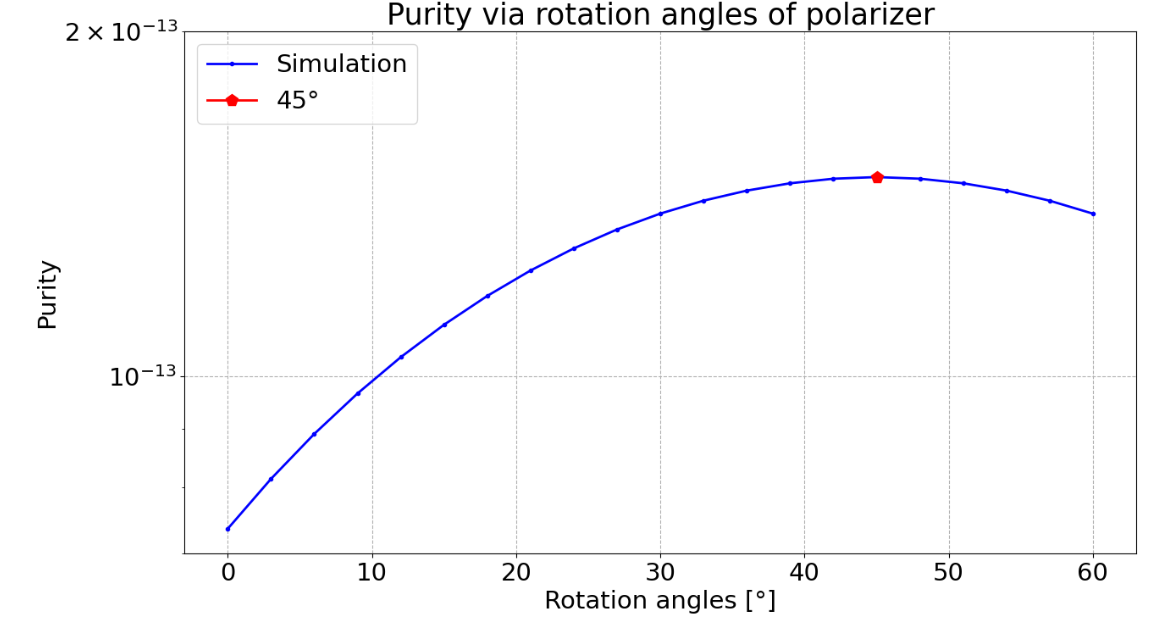
\includegraphics[width=0.95\linewidth]{figures/polarizer.png}
\caption{The linear purity simulation for polariser rotation in angular range of 0 to 60 degrees (legend: Simulation), and the calculation value with equation~(\ref{eq:polarizer}) at 45$^\circ$.}
\end{figure}

The simulated intensity of  $I_\text{para}$ aligns well with expectations, showing a reduction to half of its original value without polarizer rotation.
However, the simulated $I_\text{cross}$ intensity remains largely unchanged, thereby doubling the linear polarization purity to 1.5$~\times~10^{-13}$, as shown in Fig.~\ref{fig:polarizer}.
Generally, when rotating the polarizer across a range from 0 to 60$^\circ$, purity values vary, starting at 7.35$~\times~10^{-14}$ at 0, increasing and then decreasing after reaching a peak of 1.5$~\times~10^{-13}$ at 45$^\circ$.
This trend suggests that equation (27) holds only for a polarizer orientation of 0 and does not align with simulation data at other angles in the case of an asymmetric angular source, with Gaussian divergence in the horizontal and collimation in the vertical direction.


\todo{
DIGEST THIS: 

Start from 5th crystal, because it rotates 90 degree, so that sigma-polarization and pi-polarization are exchanged, then the sigma-polarization will be experienced a four consecutive pi-reflections, and similarly pi-polarization intensity will be experienced four consecutive sigma-reflections. Because sigma and pi-polarization are symmetry in polarizer (first 4 crystals) and analyser (last 4 crystals), so that the results should be doubled. The calculation is as following:

Case 1: 
Using your pi-reflectivity data:
( 25000 x 0.5 x 0.94$^4$ x (2.08e-6)$^4$ ) x 2 = 3.65E-18
Notes: 0.5 is additional lost in the first crystal, last factor 2 is doubled factor.

I roughly checked in my case,  the pi-polarization reflectivity is 4.15e-6, 
( 25000 x 0.5 x 0.94$^4$ x (4.15e-6)$^4$ ) x 2 = 5.79E-17.
Which is  agree with the ray-tracing data, 5.798e-17

The ray tracing data of case 2 is same as case 1, 5.798e-17
}

% -----------------------------------------------------------------
% -----------------------------------------------------------------
\section{Crystal phase-shifters}\label{sec:phasesifters}
% -----------------------------------------------------------------
% -----------------------------------------------------------------

yyyyyyy


% -----------------------------------------------------------------
% -----------------------------------------------------------------
\section{Summary and conclusions}
\label{sec:summary}
% -----------------------------------------------------------------
% -----------------------------------------------------------------

zzzzzzz


% %%%%%%%%%%%%%%%%%%%%%%%%%%%%%%%%%%%%%%%%%%%%%%%%
% %%%%%%%%%%%%%%%%%%%%%%%%%%%%%%%%%%%%%%%%%%%%%%%%

\appendix
%\section{Appendix title}

% -----------------------------------------------------------------
% -----------------------------------------------------------------
\section{Interaction with the beamline element (like in SHADOW3)}
\label{sec:S3}
% -----------------------------------------------------------------
% -----------------------------------------------------------------

The effect of the beamline element (reflection/refraction/diffraction) is applied to the beam. In SHADOW3, once the beam arrives to the element, the changes are done in three steps 
\begin{enumerate}
    \item change the incoming electric vectors to the local $\sigma$ and $\pi$ directions.
    \item multiplication of the electric fields by the reflectivities $R_\sigma$ and $R_\pi$ and change the phases accordingly.
    \item modify the outcoming electric field to guarantee the orthogonality with the output (reflected/refracted/diffracted) direction.
\end{enumerate}

% -----------------------------------------------------------------
\subsection{Modifications of electric fields in ``local'' o.e.}
\label{sec:localoe}
% -----------------------------------------------------------------
% -----------------------------------------------------------------


The physics of the X-ray reflection and diffraction in an optical surface affects in a different way 
the {\it local} parallel ($\sigma$) and perpendicular ($\pi$) components. The ``local'' parallel component
is a vector that sits on the o.e. surface and it is not coincident with the incident $\vec{E}_\sigma$.
Therefore, one must calculate the ``local'' $\vec{u}'_\sigma$ and $\vec{u}'_\pi$ vectors that verify
1) they are orthogonal to $\vec{v}$ and ii) $\vec{u}'_\sigma$ is contained in the o.e. surface. 
This is done in the method {\tt get\_local\_directions\_sigma\_pi} of {\tt S4Beam} (listing~\ref{lst:localsigmaandpi}).

\begin{lstlisting}[caption={Method of {\tt S4Beam} to compute the local directions $\sigma$ and $\pi$ at the beamline element.}, label={lst:localsigmaandpi}, captionpos=b]
    def get_local_directions_sigma_pi(self, vNormal, vIn=None):
        """
        Given a direction N (normal to a surface), this routine calculates the "local sigma and pi"
        directions, or the unitary vectors perpendicular and parallel to the scattering plane, respectively.
        The scattering plane is defines as the plane that contains N and the ray direction vIn.

        Parameters
        ----------
        vNormal: numpy array
            An array of vectors (npoints, 3) with the normal N.
        vIn: numpy array, optional
            The array of vectors with the incident direction. If None, it uses the direction in the S4Beam.

        Returns
        -------
            tuple:
            (direction_sigma, direction_pi) the two unitary array of vectors with the sigma and pi-directions.
        """
        if vNormal.shape[1] != 3:
            raise Exception("vNormal must be an array of vectors (npoints, 3).")

        if vIn is None: vIn = self.get_columns([4, 5, 6]).T

        E_S = self.get_columns([7, 8, 9]).T
        E_P = self.get_columns([16, 17, 18]).T

        # ! * ... we have to compute
        # ! * some angles, namely the sine of the incidence angle and the sine
        # ! * of the A vector with the normal. Also, the polarized light is
        # ! * treated as a superposition of two orthogonal A vectors with the appropriate
        # ! * phase relation. These two incoming vectors have to be resolved into the
        # ! * local S- and P- component with a new phase relation.
        # ! * A_VEC will be rotated later, once the amplitude will have been determined.
        #      	CALL	CROSS 	(VVIN,VNOR,AS_TEMP)	! vector pp. to inc.pl.
        #      	IF (M_FLAG.EQ.1) THEN
        # 	        CALL	DOT	(AS_VEC,AS_VEC,AS2)
        # 	        CALL	DOT	(AP_VEC,AP_VEC,AP2)
        # 	        IF (AS2.NE.0)	THEN
        #              	 DO 499 I=1,3
        #  499   	            AS_TEMP(I) = AS_VEC(I)
        # 	        ELSE
        # 	             DO 599 I=1,3
        #  599	            AS_TEMP(I) = AP_VEC(I)
        # 	        END IF
        #      	END IF
        #      	CALL	NORM  	(AS_TEMP,AS_TEMP)	! Local unit As vector
        # CALL	CROSS	(AS_TEMP,VVIN,AP_TEMP)
        # CALL	NORM	(AP_TEMP,AP_TEMP)	! Local unit Ap vector

        v_S = vector_cross(vIn, vNormal)  # AS_TEMP
        v_Smod = vector_modulus(v_S)
        mask = (v_Smod == 0.0)
        if mask.any():
            print(">>>>>>>>>> FOUND A ZERO!!!!!")
            if v_Smod.sum() > 0:
                v_S[mask, 0] = E_S[mask, 0]
                v_S[mask, 1] = E_S[mask, 1]
                v_S[mask, 2] = E_S[mask, 2]
            else:
                v_S[mask, 0] = E_P[mask, 0]
                v_S[mask, 1] = E_P[mask, 1]
                v_S[mask, 2] = E_P[mask, 2]

        v_P = vector_cross(v_S, vIn)
        uS = vector_norm(v_S)
        uP = vector_norm(v_P)

        return vector_norm(v_S), vector_norm(v_P)
\end{lstlisting}




The electric vector can thus be expressed in two orthonormal vectors $\vec{E'}_\sigma$ and $\vec{E'}_\pi$ along these 
new directions $\vec{u'}_\sigma$ and $\vec{u'}_\pi$. Physically, it is a rotation of the old electric vectors around
the $\vec{v}$ direction to put the $\sigma$ component on top of the surface, but the rotation affect not only the 
moduli, but also the phases. The new (complex) electric vectors are build from the projection of the old ones onto the
new axes, thus originating a transformation in both moduli and phases:

\begin{eqnarray}
\vec{E'}_\sigma e^{i \phi'_\sigma} = [(\vec{E}_\sigma e^{i \phi_\sigma}).\vec{u'}_\sigma + (\vec{E}_\pi e^{i \phi_\pi}).\vec{u'}_\sigma ] 
  ~~\vec{u'}_\sigma  \\ 
\vec{E'}_\pi e^{i \phi'_\pi} = [(\vec{E}_\sigma e^{i \phi_\sigma}).\vec{u'}_\pi + (\vec{E}_\pi e^{i \phi_\pi}).\vec{u'}_\pi ] 
  ~~\vec{u'}_\pi 
\end{eqnarray}


Defining the projection of the (real) electric field components onto these versors as: 
\begin{eqnarray}
a_{11} = \vec{E}_\sigma . \vec{u'}_\sigma, ~~~~ 
a_{12} = \vec{E}_\inred{\pi} . \vec{u'}_\inred{\sigma} \nonumber \\
a_{21} = \vec{E}_\inred{\sigma} . \vec{u'}_\inred{\pi}, ~~~~
a_{22} = \vec{E}_\pi . \vec{u'}_\pi 
\end{eqnarray}

we get:
\begin{eqnarray}
\label{withphases}
\vec{E'}_\sigma e^{i \phi'_\sigma} = (a_{11} e^{i \phi_\sigma} + a_{12} e^{i \phi_\pi}) \vec{u'}_\sigma \nonumber \\ 
\vec{E'}_\pi e^{i \phi'_\pi} =    (a_{21} e^{i \phi_\sigma} + a_{22} e^{i \phi_\pi}) \vec{u'}_\pi
\end{eqnarray}

And the moduli are: 

\begin{eqnarray}
|\vec{E'}_\sigma|^2 = \vec{E'}_\sigma . \vec{E'}_\sigma^*  = 
a_{11}^2 + a_{12}^2 + 2 a_{11} a_{12} \cos(\phi_\sigma-\phi_\pi) \equiv
M_\sigma^2 \nonumber \\ 
|\vec{E'}_\pi|^2    = \vec{E'}_\pi    . \vec{E'}_\pi^*     = 
a_{21}^2 + a_{22}^2 + 2 a_{21} a_{22} \cos(\phi_\sigma-\phi_\pi) \equiv
M_\pi^2
\end{eqnarray}

Therefore we can construct the new local (real) electric fields as: 
\begin{eqnarray}
\label{final1}
\vec{E'}_\sigma = M_\sigma \vec{u'}_\sigma  \nonumber \\ 
\vec{E'}_\pi = M_\pi \vec{u'}_\pi  
\end{eqnarray}

To compute the new phases, we insert Eq.~\ref{final1} in Eq.~\ref{withphases} and get: 
\begin{eqnarray}
e^{i \phi'_\sigma} = M_\sigma^{-1} (a_{11} e^{i \phi_\sigma} + a_{12} e^{i \phi_\pi})  \nonumber \\ 
e^{i \phi'_\pi} =  M_\pi^{-1}      (a_{21} e^{i \phi_\sigma} + a_{22} e^{i \phi_\pi}) 
\end{eqnarray}

Therefore:
\begin{eqnarray}
\label{final2}
\tan{\phi'_\sigma} = \frac{Im(a_{11} e^{i \phi_\sigma} + a_{12} e^{i \phi_\pi})}
                          {Re(a_{11} e^{i \phi_\sigma} + a_{12} e^{i \phi_\pi})} = 
                          \frac{a_{11} \sin{\phi_\sigma} + a_{12} \sin{\phi_\pi}}
                               {a_{11} \cos{\phi_\sigma} + a_{12} \cos{\phi_\pi}}  \nonumber \\ 
\tan{\phi'_\pi} =  \frac{Im(a_{21} e^{i \phi_\sigma} + a_{22} e^{i \phi_\pi})}
                        {Re(a_{21} e^{i \phi_\sigma} + a_{22} e^{i \phi_\pi})} = 
                        \frac{a_{21} \sin{\phi_\sigma} + a_{22} \sin{\phi_\pi}}
                             {a_{21} \cos{\phi_\sigma} + a_{22} \cos{\phi_\pi}}
\end{eqnarray}


The code that implements Eq.~\ref{final1} and Eq.~\ref{final2} is in listing~\ref{lst:rotationelements}: 

\begin{lstlisting}[caption={Code to compute the local $\sigma$ and $\pi$ electric fields at the beamline element.}, label={lst:rotationelements}, captionpos=b]
            #
            # STEP 1: get local sigma and pi directions v_S and v_P (uS and uP unitary vectors)
            #

            uS, uP = footprint.get_local_directions_sigma_pi(vH, vIn=vIn)

            #
            # calculate the electric field in the local coordinate system
            #

            # CALL	DOT	(AS_VEC,AS_TEMP,A11)	! matrix element of rotation
            # CALL	DOT	(AP_VEC,AS_TEMP,A12)	! matrix element of rotation
            # CALL	DOT	(AS_VEC,AP_TEMP,A21)	! matrix element of rotation
            # CALL	DOT	(AP_VEC,AP_TEMP,A22)	! matrix element of rotation
            # ! ** Now recompute the ampltitude and phase of the local S- and P- component.
            # AS_NEW	= SQRT(ABS(A11**2 + A12**2 +  &
            #         2.0D0*A11*A12*COS(PHS-PHP)))
            # AP_NEW	= SQRT(ABS(A21**2 + A22**2 +  &
            #         2.0D0*A21*A22*COS(PHS-PHP)))
            # CALL	SCALAR	(AS_TEMP,AS_NEW,AS_VEC)	! Local As vector
            # CALL	SCALAR	(AP_TEMP,AP_NEW,AP_VEC)	! Local Ap vector
            # PHTS	= A11*SIN(PHS) + A12*SIN(PHP)
            # PHBS	= A11*COS(PHS) + A12*COS(PHP)
            # PHTP	= A21*SIN(PHS) + A22*SIN(PHP)
            # PHBP	= A21*COS(PHS) + A22*COS(PHP)
            # CALL	ATAN_2	(PHTS,PHBS,PHS)		! Phase of local As vector
            # CALL	ATAN_2	(PHTP,PHBP,PHP)		! Phase of local Ap vector
            # ! C
            # ! C
            # CALL	DOT	(VVIN,VNOR,SIN_VAL)	! sin(graz. ang)
            # CALL	DOT	(Q_OUT,VNOR,SIN_REF)	! sin(graz.ref.ang)

            a11 = vector_dot(E_S, uS)
            a12 = vector_dot(E_P, uS)
            a21 = vector_dot(E_S, uP)
            a22 = vector_dot(E_P, uP)

            M2_S = a11 ** 2 + a12 ** 2 + 2 * a11 * a12 * numpy.cos(PhiS - PhiP)
            M2_P = a21 ** 2 + a22 ** 2 + 2 * a21 * a22 * numpy.cos(PhiS - PhiP)

            E_local_S = vector_multiply_scalar(uS, numpy.sqrt(M2_S))
            E_local_P = vector_multiply_scalar(uP, numpy.sqrt(M2_P))

            local_PhiS = numpy.arctan2((a11 * numpy.sin(PhiS) + a12 * numpy.sin(PhiP)) , (a11 * numpy.cos(PhiS) + a12 * numpy.cos(PhiP)))
            local_PhiP = numpy.arctan2((a21 * numpy.sin(PhiS) + a22 * numpy.sin(PhiP)) , (a21 * numpy.cos(PhiS) + a22 * numpy.cos(PhiP)))
            # END OF STEP 1
\end{lstlisting}



Note that these transformations imply a polarization mixing, or not conservation of the intensity of each component during the projection ($|\vec{E'}_\sigma| \ne |\vec{E}_\sigma|$),
but the total intensity is conserved ($I=|\vec{E}_\sigma|^2+|\vec{E}_\pi|^2=
|\vec{E'}_\sigma|^2+|\vec{E'}_\pi|^2$). The phases also change.
% but the difference of thase is conserved $\Phi=\phi_\sigma-\pi_\pi=\phi'_\sigma-\phi'_\pi$ (I think, but I have not demostrated it).
The new electric vectors are orthogonal to $\vec{v}$ by constructions.

% -----------------------------------------------------------------
\subsection{Reflection/refraction in the o.e. and subsequent changes in electric vectors}
\label{sec:reflection}
% -----------------------------------------------------------------

Once the electric vectors are expressed in the o.e. local coordinates ($\vec{E'}_\sigma$ and 
$\vec{E'}_\pi$) they are multiplied by the mirror/crystal reflectivities and the phases also affected: : 
\begin{eqnarray}
 \label{reflectivities}
 \vec{E'}_\sigma^{new} = \vec{E'}_\sigma R_\sigma, \nonumber \\
 \vec{E'}_\pi^{new} = \vec{E'}_\pi R_\pi, \nonumber \\
 {\phi '}_\sigma^{new} = {\phi '}_\sigma + \Sigma_\sigma, \nonumber \\
 {\phi '}_\pi^{new} = {\phi '}_\pi + \Sigma_\pi,
\end{eqnarray}
where $R_\sigma$ and $R_\pi$ are the o.e. reflectivities and $\Sigma_\sigma$ and $\Sigma_\pi$ are the  phases added in the reflection/refraction/diffraction. 

% -----------------------------------------------------------------
\subsection{subsequent changes in electric vectors to guarantee orthogonality}
\label{sec:orthogonality}
% -----------------------------------------------------------------

The resulting electric vectors and phases after applying Eq.~\ref{reflectivities} must now hold the orthogonality relations (Eq.~\ref{ortho}) with respect to the new direction $\vec{v'}$, therefore they must be changed. 

% \color{red}
% This part was incorrectly
% done in the following code, which assumes conservation of the $\vec{E'}_\sigma$ component (except for gratings)
% and the $\pi$ component is ``mirrored''. These operations do not garantee that the resulting 
% vectors are normal to $\vec{v'}$. In some cases, in particular for $\sigma$ polarizad light onto 
% o.e.'s with mirror orientation angle $90^\circ$ can result in a loss of beam intensity in 
% subsequent changes of frames. The {\bf wrong} code was (in {\tt MIRROR1}): 
% \color{black}

% \begin{lstlisting}
% ! ** So far we have the new amplitude of the two components. We have now
% ! ** to 'reflect' A_VEC onto the mirror. For this, notice that the s-comp
% ! ** is geometrically unchanged, while the p-comp is changed. The angles
% ! ** are exchanged with respect to VVIN. Things are more complicated in
% ! ** the case of a grating, due to the vectorial nature of the diffraction,
% ! ** not treated here. We make the simplifying assumption that the
% ! ** diffraction will not change the degree of polarization. This mean that
% ! ** A_VEC will have the same components referred to the ray as before the
% ! ** diffraction. 

% VVOUT(1)	=   RAY(4,ITIK)
% VVOUT(2)	=   RAY(5,ITIK)
% VVOUT(3)	=   RAY(6,ITIK)
% ! C 
% ! C The following IF block applies only to the GRATING case.
% ! C The binormal is redefined in terms of the diffraction
% ! C plane.
% ! C
%      	IF (F_GRATING.NE.0.OR.F_BRAGG_A.EQ.1) THEN
% 	  CALL	PROJ	(VVOUT,VNOR,VTEMP)
% 	  CALL	SCALAR	(VTEMP,-2.0D0,VTEMP)
% 	  CALL	SUM	(VTEMP,VVOUT,VTEMP)
% 	  !CALL	CROSS	(VTEMP,VNOR,AS_TEMP)
% 	  CALL	CROSS_M_FLAG	(VTEMP,VNOR,AS_TEMP,M_FLAG)
%      	 IF (M_FLAG.EQ.1) THEN
% 	   CALL	DOT	(AS_VEC,AS_VEC,AS2)
% 	   CALL	DOT	(AP_VEC,AP_VEC,AP2)
% 	  IF (AS2.NE.0)	THEN
%      	    DO 899 I=1,3
%  899          AS_TEMP(I) = AS_VEC(I)
% 	  ELSE
% 	   DO 999 I=1,3
%  999	     AS_TEMP(I) = AP_TEMP(I)
%      	  END IF
% 	 END IF
%      	  CALL	NORM  	(AS_TEMP,AS_TEMP)	! Local unit As vector
% 	  CALL	CROSS	(AS_TEMP,VTEMP,AP_TEMP)
% 	  CALL	NORM	(AP_TEMP,AP_TEMP)	! Local unit Ap vector
%      	  CALL	DOT	(AS_VEC,AS_VEC,RES)
%      	  RES	=    SQRT (RES)

%      	  CALL	SCALAR	(AS_TEMP,RES,AS_VEC)
% 	  CALL	DOT	(AP_VEC,AP_VEC,RES)
% 	  RES	=    SQRT (RES)
% 	  CALL	SCALAR	(AP_TEMP,RES,AP_VEC)
%      	END IF


% CALL	PROJ	(AP_VEC,VNOR,VTEMP)
% CALL	VECTOR	(VTEMP,AP_VEC,VTEMP)
% CALL	SCALAR	(VTEMP,-2.0D0,VTEMP)

% CALL	SUM	(AP_VEC,VTEMP,AP_VEC)
% \end{lstlisting}

% \color{red}

The code simply calculates the new $\sigma$ and $\pi$ versors orthogonal to $\vec{v'}$ and affects them by the electric field moduli that do not change. 
Also, the phases are not changed. 
This guarantees that the intensity is conserved, as well as orthogonality.
The code is in listing~\ref{lst:finalorthogonality}: 


% \color{black}

\begin{lstlisting}[caption={\todo{CORRECT!!} Code to guarantee that the local $\sigma$ and $\pi$ electric fields hold the orthogonality relationships.}, label={lst:finalorthogonality}, captionpos=b]
            #
            # STEP 3
            #

            # ! Electric vectors are changed to assure orthogonality with the new direction VVOUT
            # ! To conserve intensity, the moduli of Es and Ep must not change
            # ! AS_VEC and VVOUT are not orthogonal so a projection of S and P coordinates into the
            # ! new ones do not work as it may be a component of the electric field along VVOUT
            #
            # CALL CROSS_M_FLAG  (VVOUT,VNOR,AS_TEMP,M_FLAG) ! vector pp. to inc.pl.
            # CALL DOT (AS_VEC,AS_VEC,AS2)
            # CALL DOT (AP_VEC,AP_VEC,AP2)
            #
            # IF (M_FLAG.EQ.1) THEN
            #  IF (AS2.NE.0) THEN
            #    DO I=1,3
            #      AS_TEMP(I) = AS_VEC(I)
            #    END DO
            #  ELSE
            #   DO I=1,3
            #    AS_TEMP(I) = AP_VEC(I)
            #   END DO
            #  END IF
            # END IF
            #
            # CALL NORM   (AS_TEMP,AS_TEMP) ! Local unit As vector perp to vvout
            # CALL CROSS (AS_TEMP,VVOUT,AP_TEMP)
            # CALL NORM (AP_TEMP,AP_TEMP) ! Local unit Ap vector perp to vvout
            #
            # do i=1,3
            #   as_vec(i) = as_temp(i) * sqrt(as2)
            #   ap_vec(i) = ap_temp(i) * sqrt(ap2)
            # end do

            aS = vector_modulus(E_diffracted_S)
            aP = vector_modulus(E_diffracted_P)

            v_S = vector_cross(vOut, vH) # AS_TEMP
            v_Smod = vector_modulus(v_S)
            mask = (v_Smod == 0.0)
            if mask.any():
                print(">>>>>>>>>> FOUND A ZERO!!!!!")
                if v_Smod.sum() > 0:
                    v_S[mask, 0] = E_diffracted_S[mask, 0]
                    v_S[mask, 1] = E_diffracted_S[mask, 1]
                    v_S[mask, 2] = E_diffracted_S[mask, 2]
                else:
                    v_S[mask, 0] = E_diffracted_P[mask, 0]
                    v_S[mask, 1] = E_diffracted_P[mask, 1]
                    v_S[mask, 2] = E_diffracted_P[mask, 2]

            v_P = vector_cross(v_S, vOut) # AP_TEMP

            uS = vector_norm(v_S)
            uP = vector_norm(v_P)

            E_diffracted_S[:, 0] = uS[:, 0] * aS
            E_diffracted_S[:, 1] = uS[:, 1] * aS
            E_diffracted_S[:, 2] = uS[:, 2] * aS

            E_diffracted_P[:, 0] = uP[:, 0] * aP
            E_diffracted_P[:, 1] = uP[:, 1] * aP
            E_diffracted_P[:, 2] = uP[:, 2] * aP

            # END STEP 3
\end{lstlisting}




\newpage
\referencelist{iucr}

%-------------------------------------------------------------------------
% TABLES AND FIGURES SHOULD BE INSERTED AFTER THE MAIN BODY OF THE TEXT
%-------------------------------------------------------------------------

\end{document}                    % DO NOT DELETE THIS LINE
%%%%%%%%%%%%%%%%%%%%%%%%%%%%%%%%%%%%%%%%%%%%%%%%%%%%%%%%%%%%%%%%%%%%%%%%%%%%%%

